% !TEX encoding = UTF-8
% !TEX program = pdflatex
% !TEX spellcheck = it_IT

\documentclass[a4paper, 11pt]{article}

% sintassi
\usepackage[T1]{fontenc}
\usepackage[utf8]{inputenc}
\usepackage[english]{babel}
\DeclareUnicodeCharacter{00A0}{~}
\usepackage{fullpage}
%\usepackage[cochineal]{newtxmath}
%\usepackage{crimson,verbatim}
\usepackage{textcomp}
\usepackage{color,soul,hyperref,mwe}

% matematica e chimica

\usepackage{siunitx,amsmath,bm,chemfig}
\newcommand{\ud}{\mathop{}\!\mathrm{d}}
\sisetup{detect-all,math-rm = \ensuremath}
%\usepackage{arev}
\usepackage[charter]{mathdesign}


\setatomsep{2em}

\newcommand\setpolymerdelim[2]{\def\delimleft{#1}\def\delimright{#2}} 
\def\makebraces[#1,#2]#3#4#5{% 
\edef\delimhalfdim{\the\dimexpr(#1+#2)/2}% 
\edef\delimvshift{\the\dimexpr(#1-#2)/2}% 
\chemmove{% 
\node[at=(#4),yshift=(\delimvshift)] {$\left\delimleft\vrule height\delimhalfdim depth\delimhalfdim 
width0pt\right.$};% 
\node[at=(#5),yshift=(\delimvshift)] 
{$\left.\vrule height\delimhalfdim depth\delimhalfdim 
width0pt\right\delimright_{\rlap{$\scriptstyle#3$}}$};}} 
\setpolymerdelim()

% tabelle e grafica
\usepackage{booktabs,graphicx,graphbox,subfig,caption,pdfpages}
\captionsetup{font=small,
	format=hang,
	justification=centering,
	singlelinecheck=true,
	labelfont={sf,bf}	
}
\usepackage{float}
\floatstyle{plaintop}
\restylefloat{table}
\usepackage{multirow}
\usepackage{fancyhdr}
\pagestyle{fancy}
\fancyhead[LE,RO]{\textsl{\rightmark}}
\fancyhead[LO,RE]{\nouppercase{\leftmark}}
\fancyfoot[C]{\thepage}
\usepackage[margin=1in,headsep=.3in]{geometry}
\usepackage[suftesi]{frontespizio}
\usepackage{xparse}
\setlength\parindent{0pt}

\newenvironment{chapterabstract}{%
  \par\nobreak\noindent
  \textbf{\textit{Abstract}\hrulefill}\nobreak
  %\small
  \noindent\ignorespaces
}{%
  \par\nobreak\normalsize
  \vskip-\ht\strutbox\noindent
  \textbf{\hrulefill}%
}
\makeatletter
\NewDocumentCommand\headerspdf{ O {pages=-} m }{% [options for include pdf]{filename.pdf}
  \includepdf[%
    #1,
    pagecommand={\thispagestyle{fancy}},
    scale=1,
    ]{#2}}
\NewDocumentCommand\secpdf{somO{1}m}{% [short title]{section title}[page specification]{filename.pdf} --- possibly starred
  \clearpage
  \thispagestyle{fancy}%
  \includepdf[%
    pages=#4,
    pagecommand={%
      \IfBooleanTF{#1}{%
        \section*{#3}}{%
        \IfNoValueTF{#2}{%
          \section{#3}}{%
          \section[#2]{#3}}}},
    scale=.65,
    ]%
    {#5}}
\makeatother

\begin{document}


\includepdf[pages=-]{frontespizio4.pdf}

\begin{chapterabstract}

Lorem ipsum dolor sit amet, consectetur adipiscing elit. Vivamus at est non arcu dapibus eleifend. In facilisis, erat ullamcorper condimentum venenatis, magna mi consequat enim, ac faucibus velit libero ut sapien. Nam fringilla elit at magna imperdiet dapibus. Vestibulum malesuada fringilla placerat. Suspendisse potenti. Nam ac vehicula nibh, eget suscipit purus. Curabitur tempus erat id pulvinar consectetur. Etiam quis diam magna. Etiam feugiat vulputate consequat. Nulla libero ligula, tempor quis mollis in, placerat vitae nisi. Proin ornare ut eros ac rhoncus. Integer et metus non mi pharetra sagittis. Praesent dignissim erat vel magna efficitur, sed efficitur mi viverra. Interdum et malesuada fames ac ante ipsum primis in faucibus. Vivamus non ipsum non purus feugiat interdum non vel odio.

\end{chapterabstract} 

\section{Introduction}

\section{Experimental activity}

\subsection{Compounding (Internal Mixer)}

The process has been carried out with the instrument Thermo Haake Rheomix 600.\\
The processing parameters used are the following:

\begin{itemize}
\item Temperature T = $200^\circ$C
\item time t = 10 min
\item Rotation speed $\omega$ = 50 rpm
\end{itemize}

The sample used has the same composition as Plate 1 sample with a mass of $32.05$ g.

\subsection{Compression molding}

Prepared amount of polypropylene mixture has been used for compression molding process. A press by Carver has been used, as illustrated in Figure \ref{fig:press}. 
\begin{figure}[htp]
	\centering
	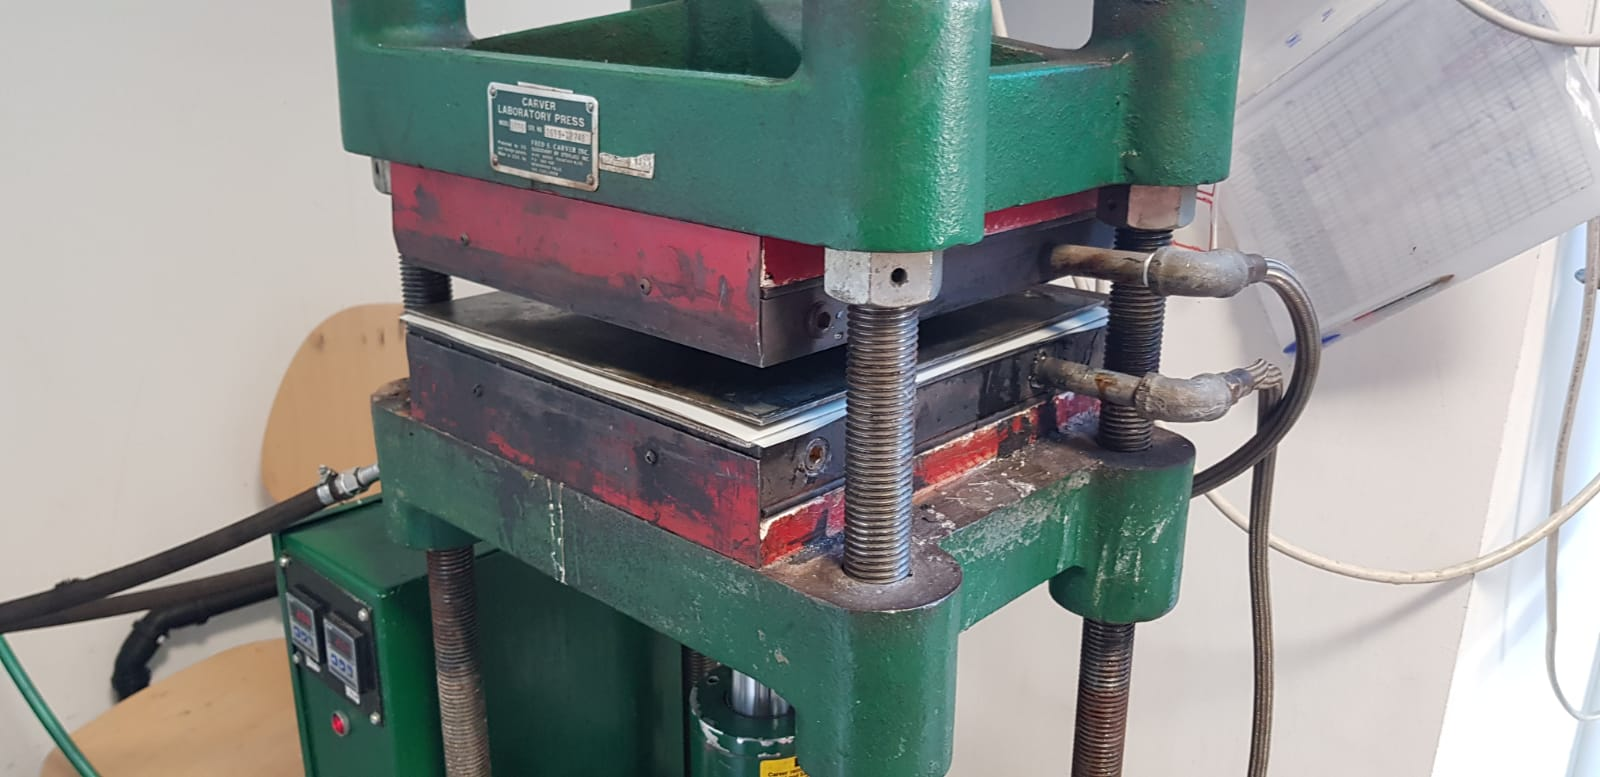
\includegraphics[scale=0.2]
	{PHOTO-2019-05-23-17-38-03.jpg}
	\label{fig:press}
	\caption{Carver press for compression molding.}
\end{figure}\\
The material to be pressed is put between two stainless steel plates, one having a frame of $12\times 12\, \text{mm}^2$ in order to produce a square plate of some mm of thickness. To avoid any adhesion with the plates, that are used to evenly distribute the pressure and to confine the melt (since the press is able to provide heat), two Mylar${^\text{\textregistered}}$ foils have been put in between the steel and the material. The press has been set to produce a pressure of 8 tons, equivalent to 5.45 MPa, in the frame. The material has undergone an heat treatment under this pressure of 200°C for 10 minutes. After this, the press has been cooled with water circulating in a refrigerating circuit inside of it and the molded piece extracted. Produced plate is then visually analyzed and weighted in order to estimate weight losses. \par 

\subsubsection{Production of dumbbell specimens}

After the analysis of the plate, this has been cut to obtain ISO 527-1BA shaped specimens, that are used in another laboratory activity.     

\section{Results and discussion}

\subsection{Compression molding}

The mold before and after pressing is reported in Figure \ref{fig:beforeafter}. 

\begin{figure}[htp]
	\centering
	\subfloat[][]
	{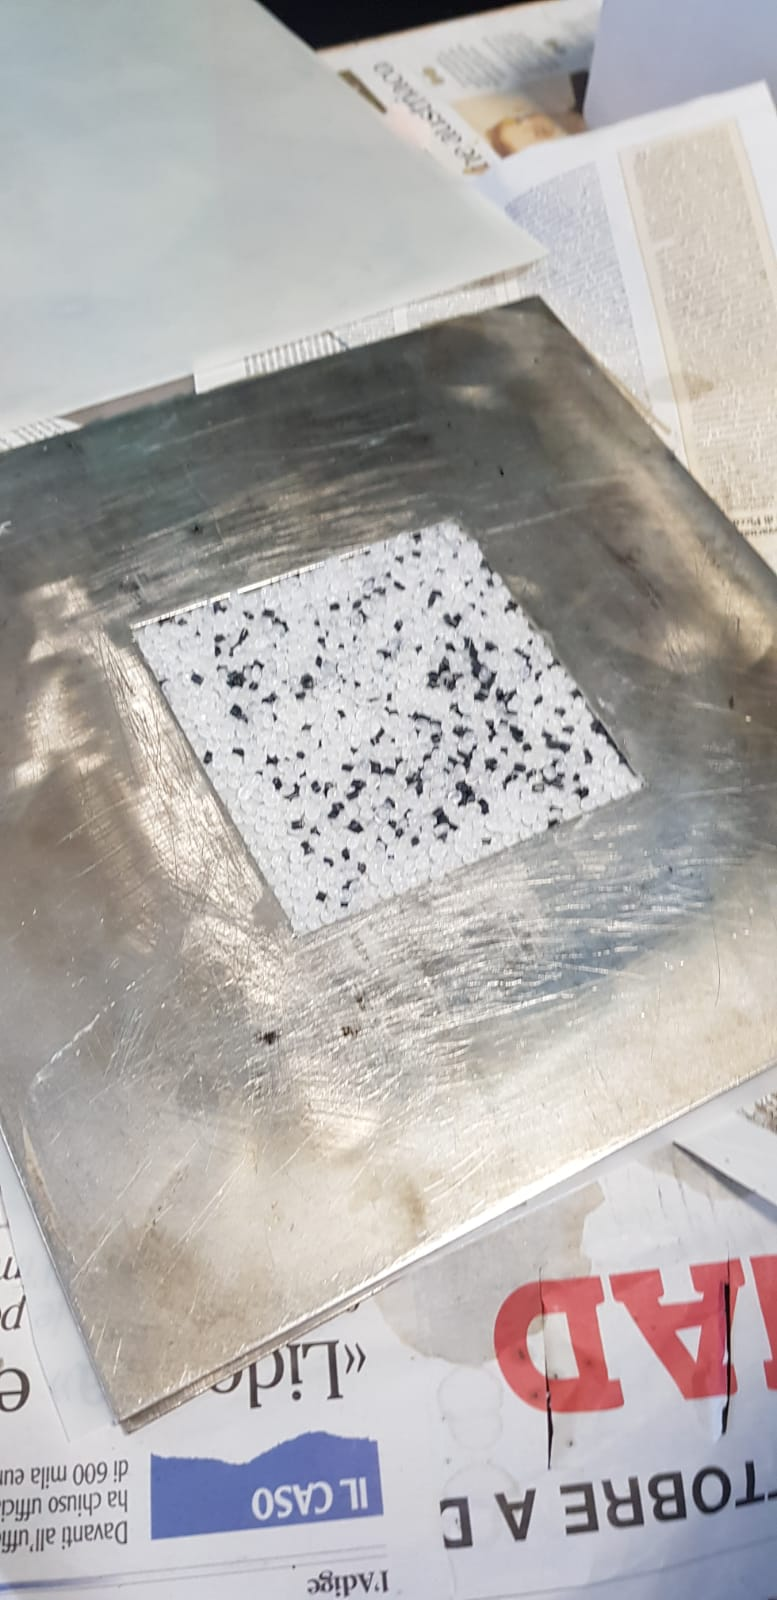
\includegraphics[scale=0.2]{PHOTO-2019-05-23-17-38-02.jpg}} \qquad 
	\subfloat[][]
	{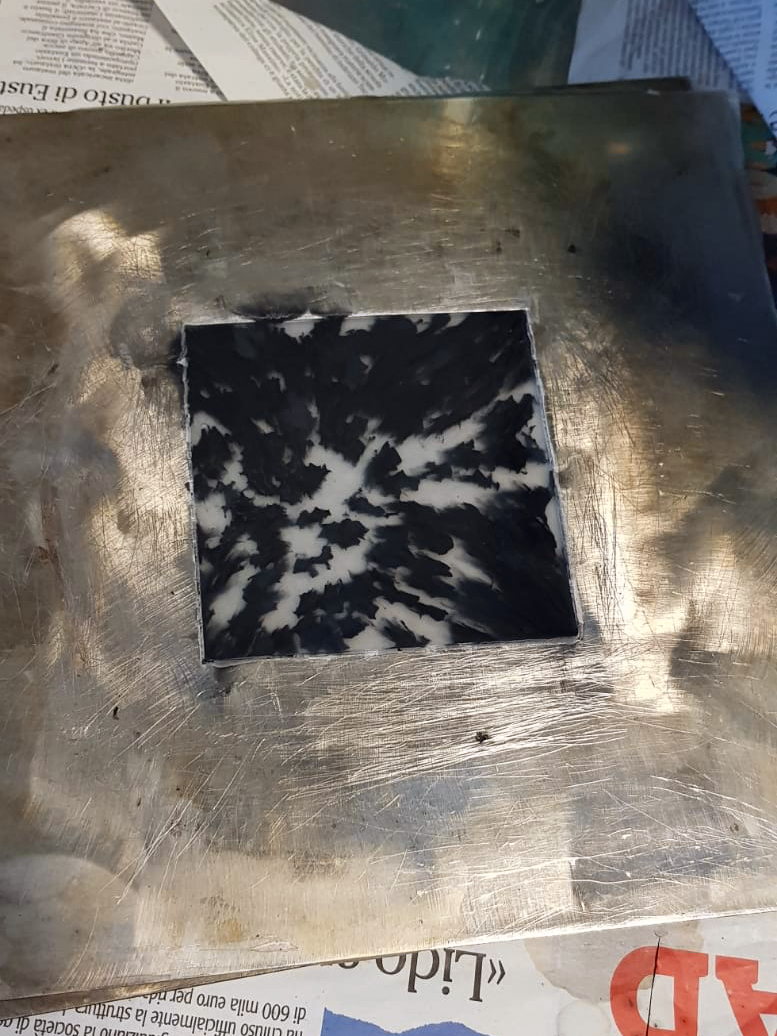
\includegraphics[scale=0.2]{PHOTO-2019-05-23-17-38-6.jpg}}
	\label{fig:beforeafter}
	\caption{Mold (a) before and (b) after compression.}
\end{figure}

The produced plate after manual mixing is illustrated in Figure \ref{fig:plate1}. 

\begin{figure}[htp]
	\centering
	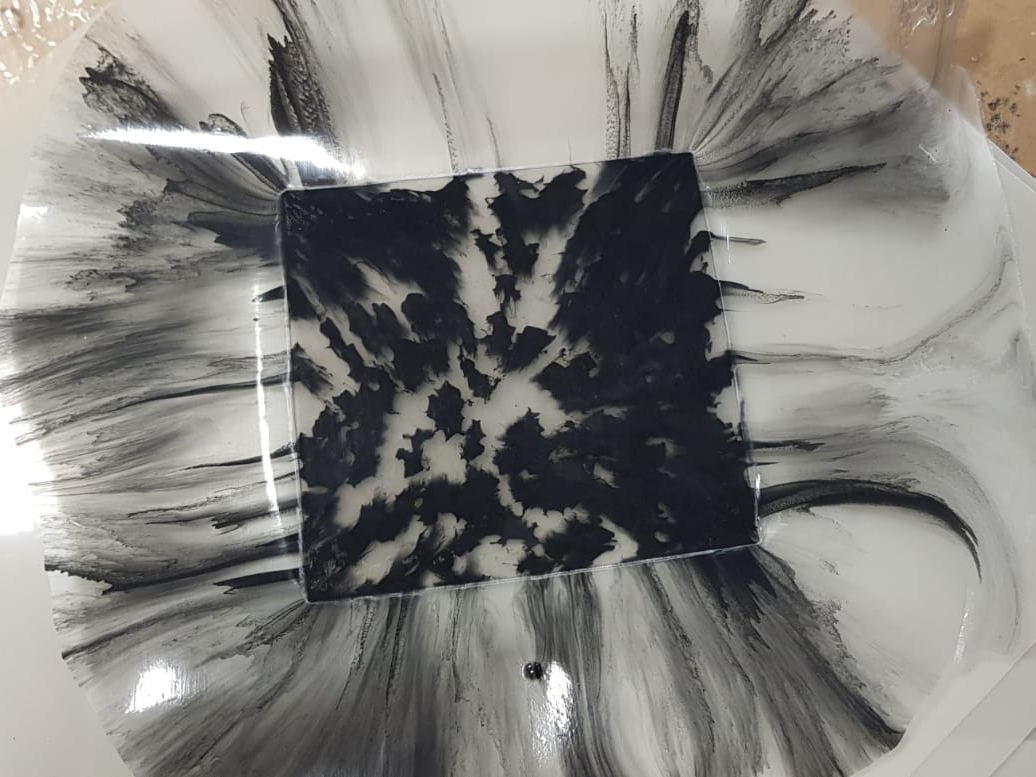
\includegraphics[scale=0.2]
	{PHOTO-2019-05-23-17-38-7.jpg}
	\label{fig:plate1}
	\caption{Plate produced in compression molding.}
\end{figure}

As it can be easily noted, the distribution of black PP in the white one is absolutely non-homogeneous, typical consequence of a manual mixing of the pellets (without any homogenization mixing in between). The other evident property of the pressed plate is the flash of melt outside of the mold: this is due to the too high amount of polymer inserted in the mold. 
The weights of the product before and after compression are reported in Table \ref{tab:weights_compression}. 

\begin{table}[htp]
	\centering
	$
	\begin{array}{ccc}
	\toprule
	\textbf{Mixture mass}\,\text{(g)} & \textbf{Plate mass}\,\text{(g)} & \textbf{Variation}\,\text{(\%)} \\
	\midrule
	34.00 & 32.50 & -4.41\\
	\bottomrule
	\end{array}
	$
	\caption{Mass of the sample before and after pressing.}
	\label{tab:weights_comparison}
\end{table}

\subsubsection{Production of dumbbell specimens}

In Figure \ref{fig:dumbbell} the dumbbell specimens produced are displayed. 
\begin{figure}[htp]
	\centering
	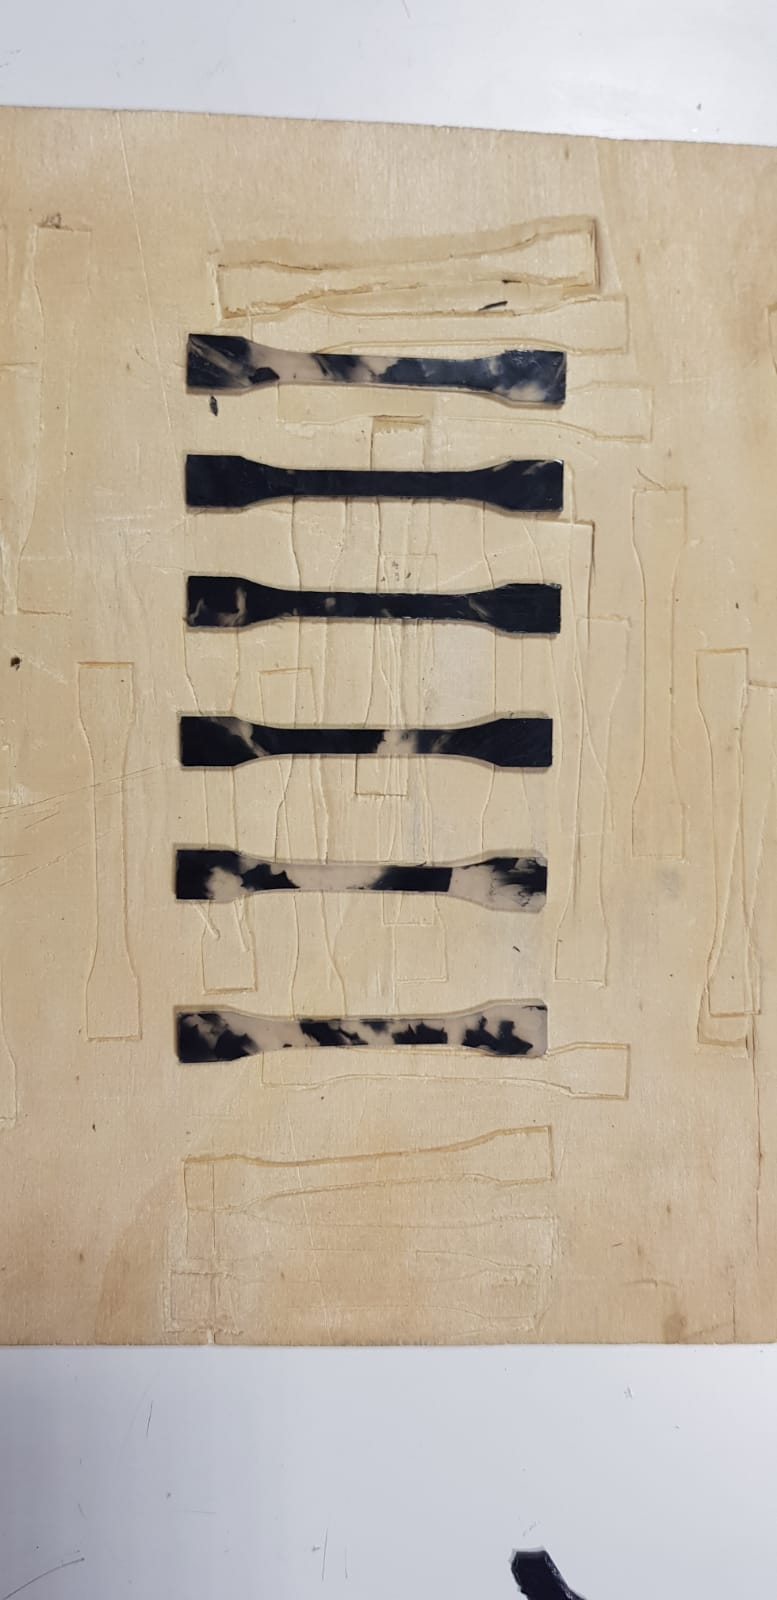
\includegraphics[scale=0.3]
	{PHOTO-2019-05-23-17-37-07.jpg}
	\label{fig:dumbbell}
	\caption{Produced specimens from compression molding plate.}
\end{figure}\\
As it can be seen, these specimens are characterized by low isotropy and homogeneity of the mixture. This will be a probable issue when mechanically testing and in resistance to flame propagation. Since the flame retardant is a weakener of strength (it introduces organics with poor adhesion and thus stress intensifiers), these specimens may have higher deformation at break than the more homogeneous ones produced in melt compounding. 

\end{document}
